\documentclass[cn]{homework}

\title{第八次作业}

\begin{document}
    \maketitle

    \problem
    由于
    \[t=\frac{\sum_{t=1}^Ty_{t-1}\varepsilon_t}
    {\hat\sigma\sqrt{\sum_{t=1}^Ty_{t-1}^2}}
    =\frac{T^{-1}\sum_{t=1}^Ty_{t-1}\varepsilon_t}
    {\hat\sigma\sqrt{T^{-2}\sum_{t=1}^Ty_{t-1}^2}}\]
    考虑到
    \[\begin{aligned}
        T^{-1}\sum_{i=1}^Ty_{t-1}\varepsilon_t
        &\Rightarrow\frac{1}{2}\sigma^2 [W^2(1)-1]\\
        T^{-2}\sum_{t=1}^Ty_{t-1}^2
        &\Rightarrow\sigma^2\int_0^1W^2(r)\diff r
    \end{aligned}\]
    同时由于$\hat\sigma^2$为$\sigma^2$的最小二乘估计,
    具有$\sqrt{T}$的收敛速度,于是具有一致性,
    进一步$\hat\sigma$弱收敛于$\sigma$,即
    \[\hat\sigma\Rightarrow\sigma\]
    因此
    \[t\Rightarrow\frac{W^2(1)-1}{2\sqrt{\int_0^1W^2(t)\diff r}}\]

    

    \problem
    不妨设$Y_0=0$,
    \[Y_t=Y_{t-1}+\varepsilon_t,\quad
    \varepsilon_t\overset{\text{i.i.d.}}\sim\mathcal N(0,\sigma^2)\]
    分别选择$\sigma^2=1,4$,
    模拟如\cref{fig:simulation}。
    \begin{figure}[h]
        \centering
        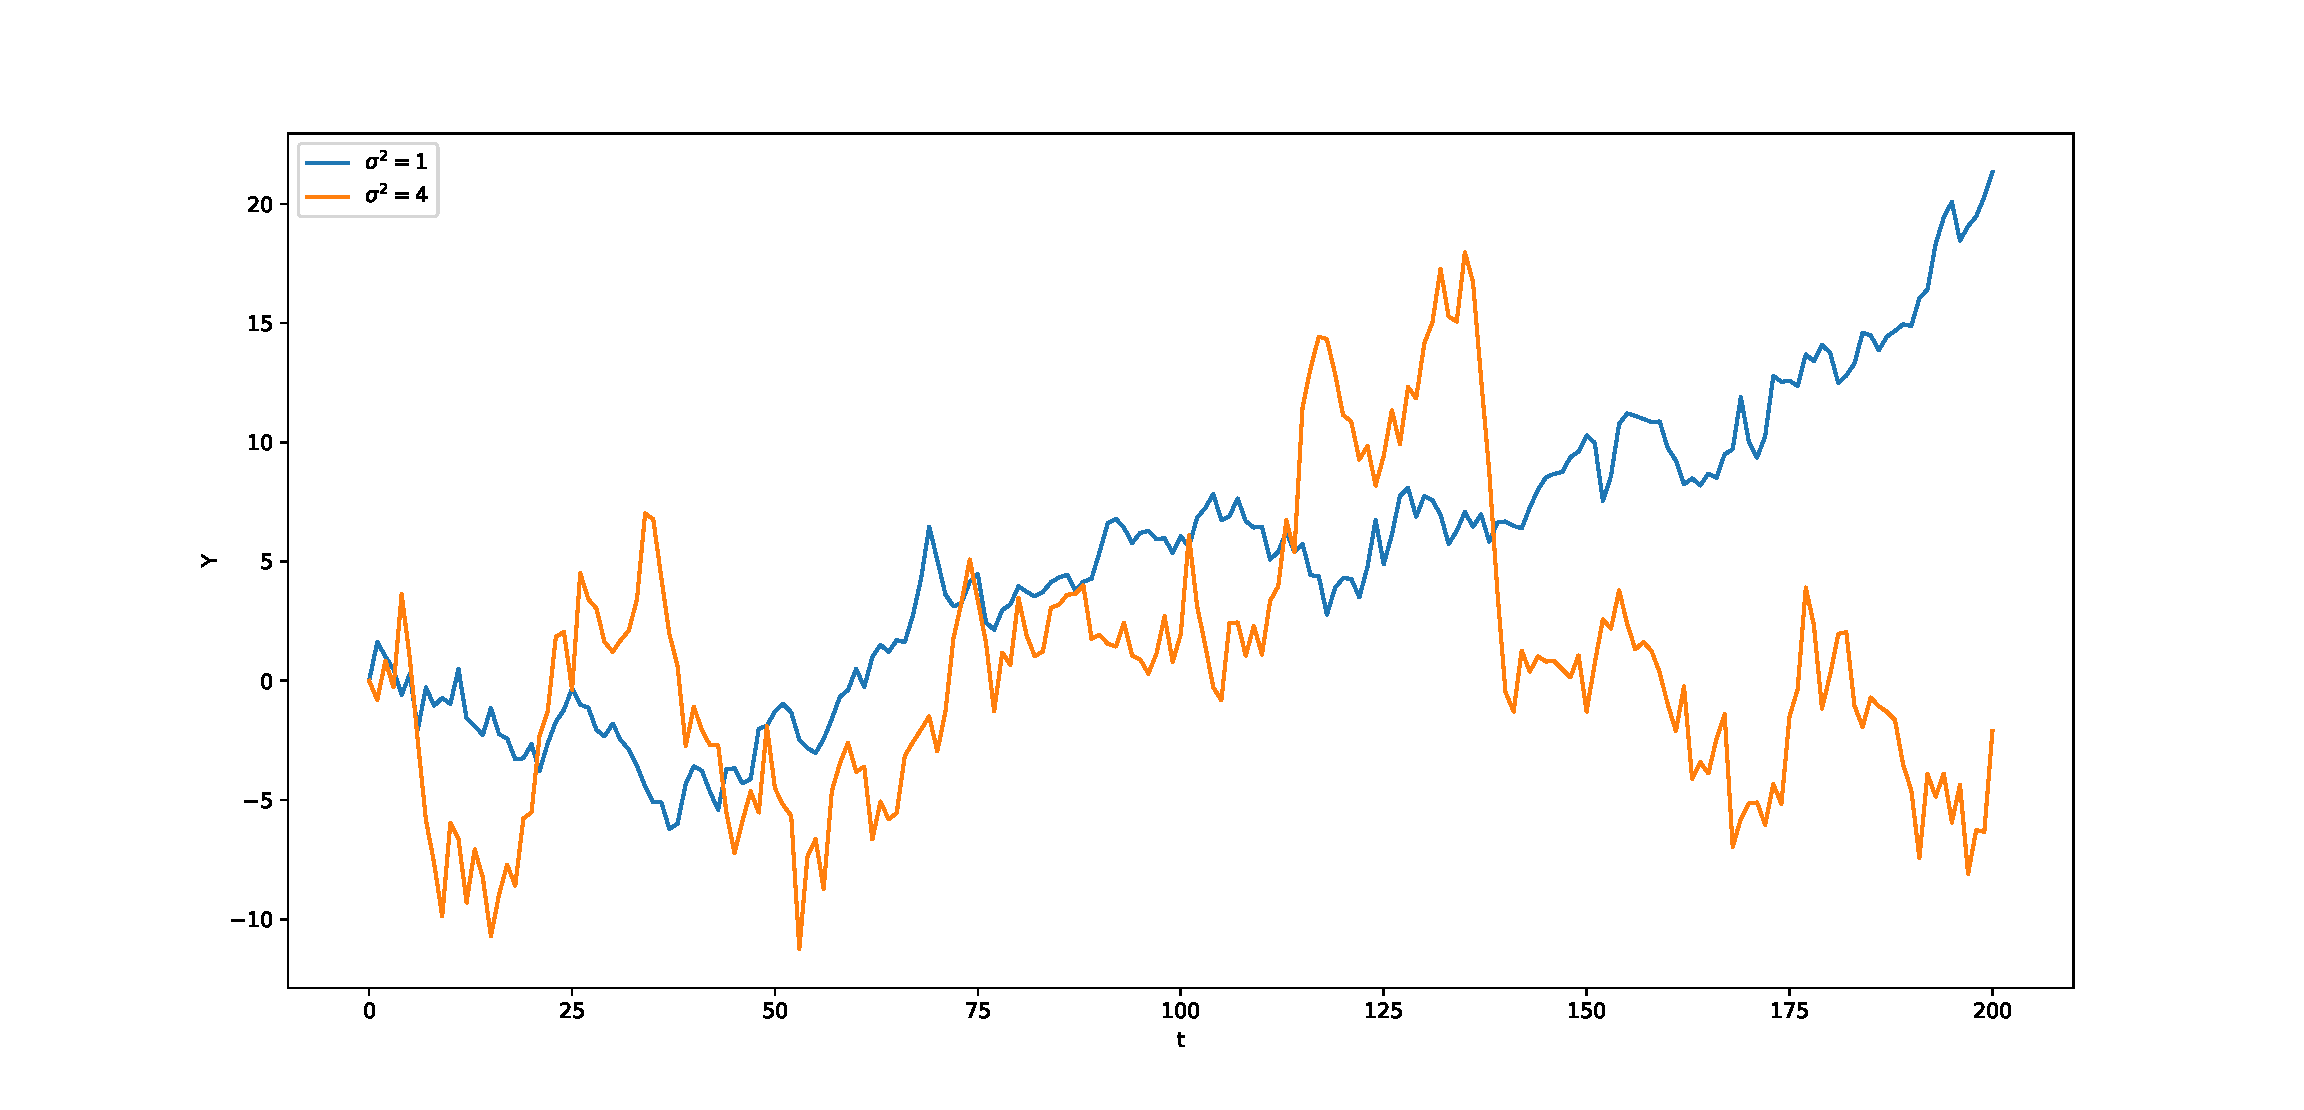
\includegraphics[width=\linewidth]{simulation}
        \caption{随机游走模拟}
        \label{fig:simulation}
    \end{figure}

    \newpage
    \appendix
    \section{随机游走代码(Python)}
    \lstinputlisting[language=Python]{simulation.py}
\end{document}